\section{Evaluierung}
Die Nutzung einer verteilten TensorFlow Umgebung zeigt deutliche Performance Vorteile. Bei der im letzten Kapitel entwickelte Anwendung führen Arbeiter einfache Berechnungen durch und aktualisieren nach jeder Iteration die Variablen auf dem Parameterserver. Bei dieser Anwendung verkürzt sich jedoch die Ausführungszeit nicht, da die Berechnung zu wenig Zeit in Anspruch nimmt und die Anzahl an Iterationen vorgegeben ist. Es ist aber zu sehen, dass wenn mehr als ein Arbeiter eingesetzt wird, sich mit jedem zusätzlichen Arbeiter sich das Ergebnis der Berechnung verbessert. D.h. wenn anstatt einem Arbeiter zwei Arbeiter verwendet werden würden, bräuchten wir pro Arbeiter nur die Hälfte an Iteration und somit die halbe Zeit, um das selbe Ergebnis zu erhalten. Um dies zu demonstrieren, können wir die Anwendung mit  unterschiedlicher Anzahl an Arbeitern starten und manuell die Anzahl an Iteration anpassen. Folgendes Ergebnis hat sich dabei ergeben:

\begin{itemize}
	\item Ein Arbeiter und ein Parameterserver:
	\begin{itemize}
		\item Die Anzahl an Iterationen für eine Session wurde auf 1000 gesetzt:
		\item Ergebnis:
		\vspace{-2mm}
			\begin{figure}[!h]
				\centering
				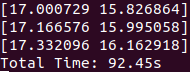
\includegraphics[width=0.5\linewidth]{Pictures/1worker1ps}
				\caption{Ein Arbeiter und ein Parameterserver}
				\label{fig:1worker1ps}
			\end{figure}
		\vspace{-5mm}
	\end{itemize}
	\item Ein Arbeiter und zwei Parameterserver:
	\begin{itemize}
		\item Die Anzahl an Iterationen für eine Session wurde auf 500 gesetzt:
		\item Ergebnis:
		\vspace{-2mm}
			\begin{figure}[!h]
				\centering
				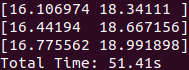
\includegraphics[width=0.5\linewidth]{Pictures/2worker1ps}
				\caption{Ein Arbeiter und zwei Parameterserver}
				\label{fig:2worker1ps}
			\end{figure}
		\vspace{-5mm}
	\end{itemize}
	\item Ein Arbeiter und drei Parameterserver:
	\begin{itemize}
		\item Die Anzahl an Iterationen für eine Session wurde auf 333 gesetzt:
		\item Ergebnis:
		\vspace{-2mm}
			\begin{figure}[!h]
				\centering
				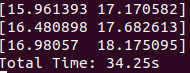
\includegraphics[width=0.5\linewidth]{Pictures/3worker1ps}
				\caption{Ein Arbeiter und drei Parameterserver}
				\label{fig:3worker1ps}
			\end{figure}	
		\vspace{-5mm}		
	\end{itemize}
\end{itemize}

Dies zeigt, dass durch das verteilen der Anwendungen auf mehrere Arbeiter können Berechnungen parallel durchgeführt werden, wodurch sich die Performance verbessert.